%====================================================================
\frame{\frametitle{Self-exciting exponential Hawkes process} \label{back:Hawkes}

  $$
  \lambda(t)= \lambda_0 + a \underset{T_k < t}{\sum} e^{-b(t-T_k)}
  $$
  \paragraph{Self exciting:} 
  Each event increases the probability of observing another event
  
  \bigskip \bigskip \pause
  \begin{tabular}{cc}
    \hspace{-.04\textwidth}
    \begin{tabular}{p{.4\textwidth}}
%       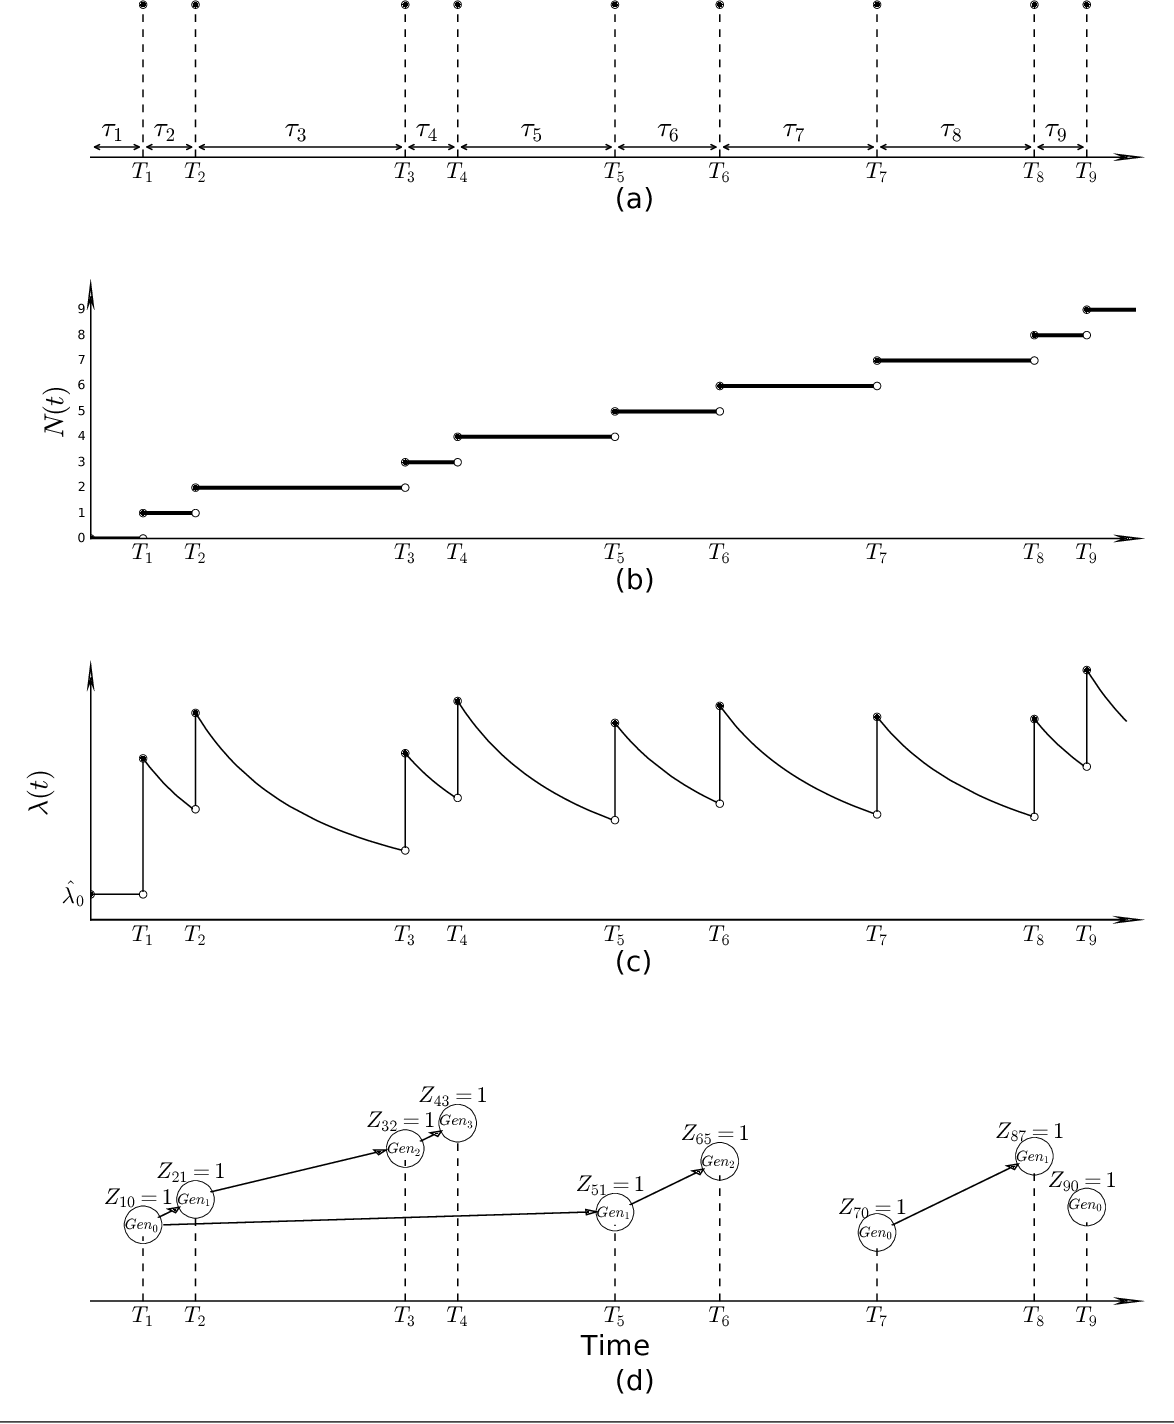
\includegraphics[width=.4\textwidth, trim=0 450 0 0, clip=]{\figcp/Bon24-Hawkes-Fig3}
      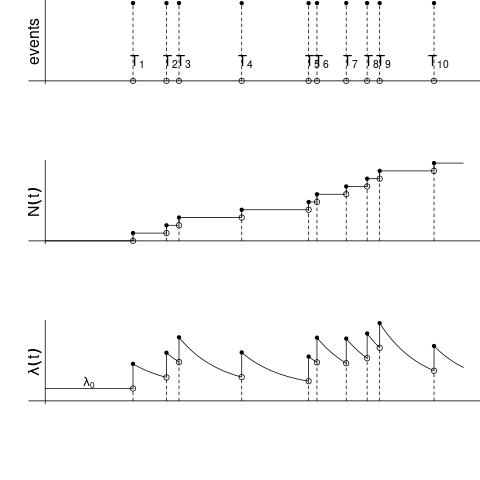
\includegraphics[width=.45\textwidth, trim=0 0 0 0, clip=]{\figcp/FigHawkes-intensity}
    \end{tabular}
    & 
%     \hspace{-.05\textwidth}
    \begin{tabular}{p{.55\textwidth}}
      \begin{itemize}
        \setlength{\itemsep}{.75\baselineskip}
        \item Exponential kernel function \emphase{$h(t)= a e^{-b t}$}
        \item \emphase{$a \geq 0$} to ensure that $\lambda$ is non negative 
        \item \emphase{$a/b <1$} to ensure stationarity
        \item Applications: sismology, epidemiology, vulcanology, neurosciences, ecology, ...
        \goto{sec:Hawkes}
      \end{itemize}
      ~ \\ ~ \\~ \\
    \end{tabular}
  \end{tabular}  
  

}

